Para poder utilizar un modelo, es necesario ajustarlo y construir alrededor de
él la interface con la cual interactuará con el usuario final. No podemos
esperar que el cito-tecnólogo tenga los conocimientos suficientes de
programación para usar el modelo de manera directa.

Implementar se refiere a tomar el modelo y convertirlo en un sistema de software
capaz. También se refiere a la forma en que el sistema será usado por el
usuario. Se refiere a las disposiciones técnicas para hacer llegar el modelo a
donde va a ser usado y se constituye de disciplinas como la ingeniería de
software, redes computacionales e internet o hardware y electrónica. 

Este concepto puede ir desde programar una interface sencilla basada en terminal
para su utilización por usuarios con conocimientos computacionales o integrado
en sistemas de software ya existentes dentro de una organización; hasta todo un
sistema web capaz de ser usado mediante el escritorio o un dispositivo móvil.
Otras implementaciones existen para poder usar el modelo en un
\emph{Smartphone} de forma nativa o en dispositivos de hardware creados
específicamente para tal fin.

Es importante mantener criterios de usabilidad bastante altos mediante el diseño
de interfaces fáciles de usar. Por ejemplo en \emph{software} que será integrado
en sistemas más grandes, diseñar Application Programming Interfaces
(\hyperlink{abbr}{API}\nomenclature{API}{Application Programming Interface})
adecuadas y en sistemas dirigidos a un usuario final, \hyperlink{abbr}{GUI}s
sencillas y que conformen buenas prácticas de User eXperience \hyperlink{abbr}{UX}.

En la \autoref{fig:logo} tenemos el logo creado para el software que será
llamado \emph{ConvoPap: Sistema inteligente de diagnóstico cervical}.

\begin{figure}[H]
    \centering
    \includegraphics[width=0.6\textwidth]{capitulo_sdac/logo}
    \caption{Nombre, logo y eslogan del sistema}\label{fig:logo}
\end{figure}

\subsection{Determinar plataforma final}
La elección de la plataforma final rige todo el desarrollo tanto del sistema
como de la siguiente fase. Para definirla, debemos de hacer un análisis
minucioso de las condiciones de uso final como el lugar o las restricciones
computacionales; también es importante retroalimentarse con el usuario final
para hacer una lista de demandas y casos de uso y poder resolverlas todas con un
solo sistema.

Existen muchos tipos de plataformas finales y dependen de como será usado
el sistema. 

\begin{itemize}
    \item{\textbf{Local: }} Se crea un programa de software tradicional y se usa
    mediante el escritorio del sistema operativo popular del momento. Tiene la
    desventaja que no existe solo un sistema operativo y se tendrían que crear
    versiones específicas para cada uno, esto incluye también los cambios de
    versiones entre estos.
    \item{\textbf{La nube: }} Es una forma muy versátil de implementar un modelo
    ya que la nube permite acceso a través del escritorio mediante un explorador
    de internet o mediante \hyperlink{abbr}{API}s que pueden ser consumidos por
    dispositivos móviles, programas de software u otros sistemas externos.
    \item{\textbf{Móvil: }} Esta forma difiere de la anterior en que el
    procesamiento se hace dentro del móvil y no en la nube. Permite desplegar
    modelos ligeros en dispositivos como \emph{smartphones} o \emph{tablets} que
    son usados masivamente en nuestra sociedad moderna. Esto permite el análisis
    de datos que son muy pesados para ser transmitidos mediante redes móviles,
    como imagen o video.
    \item{\textbf{Embebido: }} Tradicionalmente, para aplicaciones específicas
    dentro de la industria, se desarrollaban dispositivos de hardware de uso
    específico. En la actualidad, los \hyperlink{abbr}{SE}s permiten implementar
    modelos en situaciones especializadas sin tener que recurrir a un desarrollo
    caro y tardado. Aunque hay que tener consideraciones sobre el rendimiento.
\end{itemize}

\subsubsection{Condiciones de uso}

Como mencionamos anteriormente, debemos de generar una solución capaz de ser
usada dentro de un laboratorio de análisis citológico por un experto
cito-tecnólogo para poder asistirlo a clasificar células dentro de un examen
\hyperlink{abbr}{PAP} mediante el uso de un microscopio.

En esas condiciones es difícil implementar una plataforma local. Ya que se
debería programar un software específico para ser usado en el sistema operativo,
comúnmente \emph{Windows}. Esto no solo conlleva una complejidad extra puesto
que hay distintas versiones en el mercado y habría que adecuar el sistema a cada
una de ellas. También tendríamos que desarrollar el software tanto en
\emph{macOS} o \emph{Linux}. Otro problema es que tanto \emph{Windows} como
\emph{macOS} son de paga y esto incurriría en costos extra.

El uso de la nube también se descarta puesto que se tienen que analizar grandes
volúmenes de datos pesados difíciles de transmitir con la rapidez necesaria
mediante redes inalámbricas o cableadas. Inicialmente transmitiremos imágenes
pero posteriormente se planea transmitir video para una clasificación en tiempo
real.

El uso de un \emph{Smartphone} o \emph{tablet} dentro del laboratorio
citológico es algo viable. El problema radica en que también estos dispositivos
tienen dos tipos distintos de sistema operativo lo que complica el desarrollo.
Así mismo, la variedad de modelos disponibles en el mercado hace que sea
complejo estandarizar el sistema; no todas las personas tienen un teléfono con
la potencia necesaria para correr modelos de \hyperlink{abbr}{DL}. 

La plataforma debe eliminar estos problemas mientras se mantiene a un bajo
costo. También su uso debe ser sencillo, de preferencia mediante interfaces
táctiles y tiene que ser de tamaño pequeño y bajo uso energético para poder ser
desplegada dentro de un laboratorio.

\subsubsection{Plataforma}

En la actualidad los \hyperlink{abbr}{SE}s difieren de los tradicionales en que
ya vienen integrados dentro de una placa pequeña que incluye todas las
conexiones necesarias para ser usada en muchísimas aplicaciones como captura de
imagen, lectura de sensores o inclusive como computadora personal

Se consideraron los \hyperlink{abbr}{SE}s como plataforma final debido a que
cumplen con las siguientes características:

\begin{enumerate}
    \item{\textbf{Bajo costo: }} Estos dispositivos difícilmente cuestan más de
    \$100 dólares.
    \item{\textbf{Sin licencias: }} La mayoría trabajan con \emph{Linux} o
    \emph{Android} que son sistemas operativos libres y sin costo.
    \item{\textbf{Múltiples puertos: }} Cuentan con muchas conexiones USB, HDMI,
    o Ethernet pero también con puertos especializados como el GPIO para
    sensores o el bus CSI para cámaras.
    \item{\textbf{Bajo poder: }} Rara vez requieren fuentes de poder grandes y
    estorbosas. Se pueden alimentar con un pequeño cargador de 5v o inclusive el
    de un celular o batería externa.
    \item{\textbf{Popularidad: }} Existe mucha documentación y ejemplos del uso.
    En internet se pueden encontrar diseños, códigos así como soluciones a
    problemas típicos de implementación.
\end{enumerate}

El poder computacional no solo es crucial en la fase de entrenamiento de una
\hyperlink{abbr}{ConvNet}, sino también lo es durante el despliegue del modelo a
su uso final. Un modelo lento resulta poco práctico, debito a esto el
rendimiento debe ser uno de los enfoques principales.

En un laboratorio citológico es difícil poder encontrar el poder necesario para
desplegar una solución basada en \hyperlink{abbr}{DL}. Otra restricción que se
presenta radica en la poco practicidad de implementar soluciones basadas en la
nube, debido al gran volumen de datos que representan las imágenes y video, por
lo que subirlas a un sistema remoto incide negativamente en el rendimiento de la
solución final. 

Es por ello que se recurrió al uso de los \hyperlink{abbr}{SE} para desplegar la
solución en las condiciones necesarias para maximizar su uso. Hasta hace unos
meses, se tuvo la idea de desplegar el modelo dentro de un \hyperlink{abbr}{SE}
llamado \emph{Raspberry Pi}. Sin embargo, en Marzo de 2019, Nvidia lanzó al
mercado un \hyperlink{abbr}{SE} conocido como \emph{Jetson Nano}
(\autoref{fig:jetson}), basado en las potentes y caras soluciones que ofrece
Nvidia para el mercado de los carros autónomos, pero enfocado a un público con
restricciones de presupuesto o que buscan ligereza.

\begin{figure}[H]
    \centering
    \includegraphics[width=0.6\textwidth]{capitulo_marcoteorico/jetson}
    \caption{Nvidia Jetson Nano}\label{fig:jetson}
\end{figure}

En la \autoref{fig:jetsoncomp} vemos el rendimiento comparado entre tres
distintas soluciones: Coral de Google, Raspberry Pi más un módulo neural de
Intel y Jetson Nano. Como podemos ver, en la mayoría de las arquitecturas
neuronales Jetson Nano ofrece un mejor rendimiento. Las arquitecturas VGG19 y
Unet resultarán cruciales en el desarrollo de esta tesis. 

\begin{figure}[H]
    \centering
    \includegraphics[width=\textwidth]{capitulo_marcoteorico/jetson_comparison}
    \caption{Comparativa entre tres SE}\label{fig:jetsoncomp}
\end{figure}

Jetson Nano fungirá como cerebro en la creación de un dispositivo de hardware
que despliegue un modelo de \hyperlink{abbr}{ConvNet} para la clasificación de
células cérvico-uterinas. Que contará en primera instancia una cámara para
capturar imagen y video de un microscopio y de una pantalla táctil para su fácil
operación. Este se conectará a un microscopio mediante un adaptador que será
impreso en 3D. Lo que conformará el \hyperlink{abbr}{SDAC} y solución final.

Jetson Nano cuenta como un \hyperlink{abbr}{GPU} integrado optimizado para
    realizar las operaciones de álgebra lineal requeridas para el cómputo dentro
    de la \hyperlink{abbr}{ConvNet}. Este dispositivo creado por la empresa
    Nvidia, salió a la venta al público tan solo 5 meses antes de ser aprobada
    esta tesis y se caracteriza por ser de bajo costo.~\cite{Long2019}

Como plataforma se seleccionó, el \hyperlink{abbr}{SE} de Nvidia Jetson Nano. El
cual usa una distribución de \emph{Linux} especialmente mejorada por Nvidia para
aplicaciones de \hyperlink{abbr}{IA}. 

\subsection{Adecuar modelo para despliegue}
Ajustar un modelo puede ser tan sencillo como tomar los coeficientes de una
regresión lineal, extraer los pesos de una \hyperlink{abbr}{RNA} o aplicar
optimizaciones para poder desplegar el modelo en lugares con bajo poder
computacional. En estos casos es muy importante tener en cuenta la eficiencia en
la inferencia en restricciones de procesamiento, memoria, almacenamiento o
poder.

Cuantizar o \emph{Quantization} es el proceso de reducir el número de bits
necesario para representar un número. Convierte el modelo a uno de tamaño
reducido mientras mejora la eficiencia, aunque esto incurre en una degradación
en el rendimiento. 

La \autoref{tabla:cuantizacion} muestra los tres tipos disponibles para el
modelo. Habría que hacer una prueba de rendimiento entre ellas para determinar
cual es la que confluye mejor rendimiento con eficiencia. Por la naturaleza de
la plataforma, que cuenta con un \hyperlink{abbr}{GPU}, la última puede ser la
más adecuada.

\begin{table}[H]
    \centering
    \resizebox{\textwidth}{!}{%
    \begin{tabular}{@{}lll@{}}
    \toprule
    Técnica & Beneficios & Hardware \\ \midrule
    Cuantización de pesos & 4x más pequeña, 2-3x más rápida, rendimiento & CPU \\
    Cuantización a enteros & 4x más pequeña, 3x+ rápida & CPU, Edge TPU, etc. \\
    Cuantización Float16 & 2x más pequeña, aceleración potencial por GPU & CPU/GPU \\ \bottomrule
    \end{tabular}%
    }
    \caption{Tipos de cuantización para modelos de Deep Learning}\label{tabla:cuantizacion}
    \end{table}

\subsubsection{\emph{Tensorflow Lite}}

Para cuantificar y convertir nuestro modelo de \emph{Tensorflow}, utilizaremos
el módulo auxiliar \emph{Tensorflow Lite}: un framework de código abierto para
la inferencia dentro de un dispositivo.

El proceso de conversión de un modelo normal a uno capaz de ser implementado en
la Jetson Nano se divide en dos partes. El servidor se refiere al proceso de
entrenar el modelo en una computadora con \hyperlink{abbr}{GPU} y procesarlo
funciones convertidoras que tienen como salida un archivo \emph{TFLite
Flatbuffer} que ya se puede utilizar en el cliente. El intérprete de
\emph{Tensorflow Lite} se instala en el cliente, es decir, la plataforma elegida
que toma el archivo generado por el servidor para poder hacer inferencia.
\emph{Tensorflow Lite} nos permite usar el modelo tanto en \emph{iOS},
\emph{Android} y \emph{Linux} utilizando todos los tipos de procesador
(\autoref{fig:tflite}).

\begin{figure}[H]
    \centering
    \includegraphics[width=\textwidth]{capitulo_sdac/workflow.png}
    \caption{Diagrama del proceso de \emph{Tensorflow Lite}}\label{fig:tflite}
\end{figure}

\subsection{Solucionar integración}

En otros tipos de algoritmo de \hyperlink{abbr}{ML}, esta parte se refiere a
gestión para la creación de una misma \emph{app} tanto para \emph{iOS} como para
\emph{Android}, a la planeación de las \hyperlink{abbr}{API}s restful para
comunicar el modelo mediante protocolos de internet o la configuración de
sensores u otras formas de ingreso de datos e interfaces para poder usar el
modelo y convertirlo en un sistema. Es decir, las disposiciones para usar el
modelo implementado en la plataforma.

En el caso de la plataforma Jetson Nano u otro tipo de \hyperlink{abbr}{SE}, se
debe complementar el dispositivo de hardware con periféricos de entrada/salida.
En particular la pantalla táctil con la cual el cito-tecnólogo interactuará con
la plataforma y la cámara con la cual se alimentará el modelo con imágenes o
video.

\subsubsection{Dispositivo de Hardware}

El prototipo generado por el diseño conceptual será compuesto por los
componentes mostrados en la \autoref{fig:componentes}.

\begin{figure}[H]
    \centering
    \includegraphics[width=0.8\textwidth]{capitulo_marcoteorico/componentes}
    \caption{Componentes para ensamblar el SDAC}\label{fig:componentes}
\end{figure}

Jetson Nano se compone de dos partes, el módulo del procesador y la placa base.
El módulo tiene las siguientes características:

\begin{itemize}
    \item 128-core Maxwell GPU
    \item Quad-core Arm A57 processor @ 1.43 GHz
    \item System Memory  – 4GB 64-bit LPDDR4 @ 25.6 GB/s
    \item Storage  – microSD card slot (devkit) or 16GB eMMC flash (production)
    \item Video Encode – 4K @ 30 | 4x 1080p @ 30 | 9x 720p @ 30 (H.264/H.265)
    \item Video Decode – 4K @ 60 | 2x 4K @ 30 | 8x 1080p @ 30 | 18x 720p @ 30
    (H.264/H.265)
\end{itemize}

Mientras que la placa base tiene las siguientes:

\begin{itemize}
    \item 260-pin SO-DIMM connector for Jetson Nano module
    \item Video Output – HDMI 2.0 and eDP 1.4 (video only)
    \item Connectivity – Gigabit Ethernet (RJ45) + 4-pin PoE header
    \item USB – 4x USB 3.0 ports, 1x USB 2.0 Micro-B port for power or device
    mode
    \item Camera I/F – 1x MIPI CSI-2 DPHY lanes compatible with Leopard Imaging
    LI-IMX219-MIPI-FF-NANO camera module and Raspberry Pi Camera Module V2
    \item M.2 Key E socket (PCIe x1, USB 2.0, UART, I2S, and I2C) for wireless
    networking cards
    \item 40-pin expansion header with GPIO, I2C, I2S, SPI, UART signals
    \item 8-pin button header with system power, reset, and force recovery
    related signals
    \item Misc. – Power LED, 4-pin fan header
    \item Power Supply – 5V/4A via power barrel or 5V/2A via micro USB port;
    optional PoE support
\end{itemize}

Para el diseño haremos uso de la interface CSI para la cámara el cual ofrece
mejor rendimiento que los puertos USB integrados. También tenemos la posibilidad
de usar una batería externa para que el prototipo funcione de manera
inalámbrica. Gracias al procesador de arquitectura Maxwell con 128 núcleos,
podremos hacer inferencia mediante \hyperlink{abbr}{DL} sin pender rendimiento
en la captura de imagen o video.

La pantalla táctil capacitiva de siete pulgadas LCD tiene las siguientes
especificaciones. Esta servirá para interactuar con el sistema usando gestos
táctiles:

\begin{itemize}
    \item IPS screen, 1024x600 hardware resolution, configurable by software (up
    to 1920x1080).
    \item Multi languages OSD menu, for power management, brightness/contrast adjustment, etc. 
    \item 3.5mm audio jack, speaker connector, supports HDMI audio output
\end{itemize}

La cámara es modelo IMX219-77. Su gran resolución y número de megapíxeles la
hace ideal para capturar imágenes difíciles como las que se generan en un
microscopio. Tiene las siguientes características:

\begin{minipage}{\textwidth}
\begin{itemize}
    \item 8 Megapixels
    \item Sensor: Sony IMX219
    \item Resolution: 3280 × 2464
    \item CMOS size: 1/4inch
    \item Focal Length: 2.96mm
    \item Angle of View (diagonal): 77 degree
    \item Distortion: < 1\%
    \item Lens dimensions: 6.5mm × 6.5mm
\end{itemize}
\end{minipage}

Otros componentes que se le pueden agregar al sistema son una tarjeta de
\emph{WiFi} para conexión a internet o pantallas externas de alta definición
para una mejor visualización de la imagen.

Debido a que los algoritmos de \hyperlink{abbr}{DL} son computacionalmente
intensivos, generan una carga de trabajo enorme en los procesadores, lo que
incrementa el consumo de poder y, por consiguiente, la generación de calor. Un
procesador sobrecalentado reducirá su velocidad de procesamiento para bajar su
temperatura. Para evitar esto, una disipación eficaz del calor es necesaria para
mantener un rendimiento alto y constante en la inferencia. Si bien el disipador
de aluminio integrado en el módulo procesador es bastante grande, se auxiliará
de un ventilador Noctua modelo NF-A4x20 5V PWM (\autoref{fig:noctua}) que tiene
la capacidad de ser controlado por el sistema operativo instalado en Jetson Nano
para aumentar o reducir sus revoluciones según sea la temperatura, lo que lo
hace muy eficiente energéticamente. Cuenta con las siguientes características:

\begin{minipage}{\textwidth}
\begin{itemize}
    \item 40x20mm size
    \item Polarity protection
    \item Flow Acceleration Channels
    \item Integrated Anti-Vibration Pads
    \item SSO2 bearing
    \item Rotational speed (\(\pm 10\%\)) 5000 RPM
    \item Airflow \(9.4 m^{3}/h\)
    \item Acoustical noise 14,9 dB(A)
    \item Static pressure \(2.26 mm H_{2}O\)
    \item Max. input power 0.5 W
    \item Max. input current 0.1 A    
    \item Operating voltage 5 V
\end{itemize}
\end{minipage}

\begin{figure}[H]
    \centering
    \includegraphics[width=0.3\textwidth]{capitulo_sdac/noctua}
    \caption{Ventilador Noctua NF-A4x20 5V PWM}\label{fig:noctua}
\end{figure}

En la \autoref{fig:prototipo_ventilador} podemos ver la placa Jetson ya con el
ventilador Noctua integrado. Los agujeros del disipador ya estaban perforados
con las dimensiones precisas pero no contaban con estrías para asegurar el
tornillo, re recurrió al uso de una herramienta especializada para crear estas
estrías y asegurar firmemente el ventilador al disipador.

\begin{figure}[H]
    \centering
    \includegraphics[width=0.6\textwidth]{capitulo_sdac/prototipo_ventilador}
    \caption{Jetson Nano integrado con Noctua}\label{fig:prototipo_ventilador}
\end{figure}

Para conjugar todos estos dispositivos se requiere una carcasa rígida capaz de
albergarlos y protegerlos. También hay que encontrar la manera de conectar la
cámara al objetivo del microscopio. Debe tener el espacio justo con suficiente
ventilación así como los agujeros dispuestos para todos los puertos del Jetson
Nano. El adaptador de la cámara debe ser capaz de sellar perfectamente la
entrada de luz para no incidir con ruido en la toma de la imagen.

\subsubsection{Impresión 3D}

Para la creación de la carcasa y el adaptador, se decidió utilizar la impresión
3D para agilizar el proceso de prototipado. Transfiriendo la dificultad de
diseñar y crear tanto la carcasa como el adaptador en madera o plástico
termo-deformable, al tiempo que se tarda una impresora 3D en imprimir cada una
de las partes tanto del adaptador como de la carcasa.

El Centro Regional de Optimización y Desarrollo de Equipo de Orizaba fue un gran
apoyo al proveer infraestructura y mano de obra calificada para la realización
del prototipo y la impresión 3D. El centro cuenta con dos tipos de impresora 3D:

\begin{enumerate}
    \item{\textbf{Form2 de FormLabs: }}  Una impresora de resina fotopolímera
    que es curada con un rayo laser UV (\autoref{fig:resina}). Alcanza grandes
    precisiones en todos los ejes ya que el grosor del laser es ínfimamente más
    pequeño (140 micrones) que el de un filamento de plástico. Cuenta con una
    precisión de 0.050 mm.
    \item{\textbf{Pro2 Plus de Raise3D: }} Es una impresora de filamento
    plástico (\autoref{fig:plastico}) capaz de alcanzar una resolución de
    0.01mm. Es rápida que la de resina y cuenta con dos cabezales de
    alimentación de filament y permite imprimir una pieza con distintos colores,
    uno por cada rollo de filamento. 
\end{enumerate}

\begin{figure}[H]
    \centering
    \includegraphics[width=0.7\textwidth,angle=270,origin=c]{capitulo_sdac/impresora_resina}
    \caption{Impresora Form2 de resina fotopolímera}\label{fig:resina}
\end{figure}

\begin{figure}[H]
    \centering
    \includegraphics[width=0.7\textwidth]{capitulo_sdac/impresora_plastico}
    \caption{Impresora Pro2Plus de filamento plástico}\label{fig:plastico}
\end{figure}

El adaptador de cámara se compone de tres partes y fue diseñado para adaptar
dispositivos creados con Raspberry Pi usando la cámara oficial de Raspberry por
el usuario \hyperlink{https://www.thingiverse.com/luisibanez/about}{Luis
Ibanez}\footnote{\url{https://www.thingiverse.com/thing:214466}} en el sitio
\hyperlink{https://www.thingiverse.com/}{Thingiverse}. El modelo de cámara usado
con Jetson Nano difiere un poco comparado con la cámara de Raspberry, debido a
esto se tuvo que modificar el modelo para poder adaptarlo a la cámara a utilizar
utilizando el software OpenSCAD para diseño asistido por computadora. En la
\autoref{fig:adaptador_final} vemos un ejemplo del uso final del adaptador, para
acoplar la cámara al objetivo del microscopio

\begin{figure}[H]
    \centering
    \includegraphics[width=0.8\textwidth]{capitulo_sdac/adaptador_final}
    \caption{Ejemplo de uso del adaptador impreso en 3D}\label{fig:adaptador_final}
\end{figure}

\begin{minipage}{\textwidth}
    Las partes del adaptador son las siguientes:
    \begin{enumerate}
        \item El adaptador de cámara, que alojará la cámara para protección.
        \item El adaptador de cámara-microscopio, que se acoplará al otro adaptador
        para conectar la cámara seguramente al microscopio.
        \item La tapa de atrás, para evitar el paso de la luz y asegurar la cámara.
    \end{enumerate}
\end{minipage}


El primer prototipo se realizó en la impresora Form2 ya que la resina
transparente permite ver mejor como se inserta la cámara para analizar el
ajuste, ya que ambos modelos de cámara son diferentes. En la
\autoref{fig:interface_impresora_resina} se observa la interface táctil de la
impresora 3D mientras se dispone a imprimir el adaptador de la cámara.

\begin{figure}[H]
    \centering
    \includegraphics[width=0.6\textwidth]{capitulo_sdac/interface_impresora_resina}
    \caption{Interface táctil de la impresora Form2}\label{fig:interface_impresora_resina}
\end{figure}

% \begin{figure}[H]
%     \centering
%     \includegraphics[width=0.6\textwidth]{capitulo_sdac/primer_prototipo_resina}
%     \caption{Interface táctil de la impresora Form2}\label{fig:primer_prototipo_resina}
% \end{figure}

El prototipo terminado se puede ver en la \autoref{fig:primer_prototipo_resina}.
Claramente se observa la muesca del cable y la base que genera la impresora como
estructura del diseño.

\begin{figure}[H]
    \centering
    \includegraphics[width=0.6\textwidth]{capitulo_sdac/primer_prototipo_resina1}
    \caption{Interface táctil de la impresora Form2}\label{fig:primer_prototipo_resina}
\end{figure}

Podemos ver el resultado de la impresión de las tres piezas del adaptador en la
\autoref{fig:resina_adaptador}. También se proporciona la tapa trasera que
mantiene la cámara en su sitio y evitaría, en un material opaco, el paso de la
luz.

\begin{figure}[H]
    \centering
    \includegraphics[width=0.6\textwidth]{capitulo_sdac/resina_adaptador}
    \caption{Interface táctil de la impresora Form2}\label{fig:resina_adaptador}
\end{figure}

El prototipo no tuvo un ajuste perfecto debido a que el conector de cable plano
de la cámara usada está al frente mientras que en la cámara Raspberry está
atrás. Para ello se tuvo que modificar el archivo CAD del adaptador para
ajustarlo a la cámara de la Jetson Nano. Se puede observar que se trasladó la
muesca del cable a su antípoda y se horadó una brecha del lado de la nueva
muesca para alojar el conector de cable plano (\autoref{fig:adaptadores}).

\begin{figure}[H]
    \centering
    \begin{subfigure}{.5\textwidth}
        \centering
        \includegraphics[width=.7\linewidth]{capitulo_sdac/adaptador_raspberry}
        \caption{Adaptador de cámara Raspberry}
    \end{subfigure}%
    \begin{subfigure}{.5\textwidth}
        \centering
        \includegraphics[width=.7\linewidth]{capitulo_sdac/adaptador_jetson}
        \caption{Adaptador de cámara Jetson Nano}
    \end{subfigure}
    \caption{Adaptador de cámara Jetson Nano}\label{fig:adaptadores}
    \end{figure}

Una vez analizado el primer prototipo y tomadas las consideraciones para el
cambio del archivo CAD. Se procedió a imprimir otro prototipo en la impresora
Pro2 Plus. Debido a que esta puede imprimir más rápido y también a la
disponibilidad de imprimir en un material opaco a la luz visible.

%  La interface táctil de la impresora, donde muestra el tiempo
% restante, el número de capa y porcentaje del trabajo se ve en la
% \autoref{fig:interfaz_impresora_plastico}.

% \begin{figure}[H]
%     \centering
%     \includegraphics[width=0.7\textwidth,angle=270,origin=c]{capitulo_sdac/interfaz_impresora_plastico}
%     \caption{}\label{fig:interfaz_impresora_plastico}
% \end{figure}

Para el prototipo final primero se imprimió el adaptador para el objetivo del
microscopio. La impresión 3D es un proceso realizado capa por capa. En la
\autoref{fig:cabezal_impresion_plastico} vemos ambos cabezales de la impresora
3D, cada uno alimentado por un filamento de distinto color. El blanco fue usado
para la construcción de la base de impresión mientras que el negro se usó para
el adaptador mismo.

\begin{figure}[H]
    \centering
    \includegraphics[width=0.7\textwidth]{capitulo_sdac/cabezal_impresion_plastico}
    \caption{}\label{fig:cabezal_impresion_plastico}
\end{figure}

Los dos adaptadores ya terminados se muestran junto con sus bases de impresión
en la \autoref{fig:adaptadores_finales}. Del adaptador del  microscopio se
pueden notar cuatro piezas de anclaje para conectarlo al adaptador de la cámara.
En el adaptador de la cámara podemos ver la adaptación para que se acople la
cámara de Jetson Nano.

\begin{figure}[H]
    \centering
    \begin{subfigure}{.5\textwidth}
        \centering
        \includegraphics[width=.8\linewidth]{capitulo_sdac/adaptador_microscopio}
        \caption{Adaptador de cámara Raspberry}
    \end{subfigure}%
    \begin{subfigure}{.5\textwidth}
        \centering
        \includegraphics[width=.8\linewidth]{capitulo_sdac/adaptador_camara}
        \caption{Máscara}
    \end{subfigure}
    \caption{Adaptadores para conectar la cámara al microscopio}\label{fig:adaptadores_finales}
    \end{figure}

Para alcanzar el ajuste perfecto, se necesitaron cuatro prototipos. Podemos ver
como se va abriendo progresivamente la brecha para alojar el conector de cable
plano. Las tres piezas finales consisten en los dos adaptadores y en la tapa
para ajustar la cámara (\autoref{fig:adaptador_jetson}).

\begin{figure}[H]
    \centering
    \begin{subfigure}{.5\textwidth}
        \centering
        \includegraphics[width=.8\linewidth]{capitulo_sdac/prototipos}
        \caption{Adaptador de cámara Raspberry}
    \end{subfigure}%
    \begin{subfigure}{.5\textwidth}
        \centering
        \includegraphics[width=.8\linewidth]{capitulo_sdac/impresion_final}
        \caption{Piezas del adaptador final}
    \end{subfigure}
    \caption{Adaptador de cámara Jetson Nano}\label{fig:adaptador_jetson}
\end{figure}

El resultado final de la impresión para adaptar
(\autoref{fig:resultado_impresion}) tiene un ajuste perfecto en la cámara y
permite su conexión al microscopio. Debido a la falta de  un microscopio
disponible, las pruebas de ajuste y aislamiento de luz se dejarán para trabajos
posteriores.

\begin{figure}[H]
    \centering
    \includegraphics[width=0.8\textwidth]{capitulo_sdac/resultado_impresion}
    \caption{Resultado final de la impresión 3D}\label{fig:resultado_impresion}
\end{figure}

Se realizó un experimento con la impresora Form2 para la creación de la carcasa
para alojar tanto la Jetson como su pantalla. La carcasa se compone de distintas
partes y se realizó la prueba con la más grande. Esta pieza contiene la Jetson y
tiene espacio suficiente para colocar el ventilador Noctua
(\autoref{fig:carcasa_print}). Llama la atención el entramado interno que genera
el software de impresión 3D para darle soporte a la estructura mientras se
imprime.

\begin{figure}[H]
    \centering
    \includegraphics[width=0.6\textwidth]{capitulo_sdac/carcasa_impresion}
    \caption{Impresión terminada de la carcasa}\label{fig:carcasa_print}
\end{figure}

La \autoref{fig:carcasa} revela los puertos de entrada. La resina recién impresa
continua una reacción química por lo que es necesario lavarla en alcohol
isopropílico para detenerla y disolver todo resto de resina líquida que quede
sobre la superficie, posteriormente se necesita un periodo de curación mediante
rayos UV para alcanzar la integridad física normal del material; este proceso
opaca la resina lo cual dota de la pieza de un color blancuzco.

\begin{figure}[H]
    \centering
    \includegraphics[width=0.8\textwidth]{capitulo_sdac/carcasa1}
    \caption{Experimento para la impresión de la carcasa}\label{fig:carcasa}
\end{figure}

El tiempo de impresión de esta pieza fue de 17 horas. Debido a que la carcasa se
compone de piezas con un tiempo muy similar de impresión, se tuvo una
restricción de tiempo y solo se pudo imprimir el prototipo mencionado. A futuro
se realizarán más prototipos en la impresora de plástico para culminar en la
impresión de todas las piezas de la carcasa.

Un ejemplo del uso final de la carcasa se puede ver en la \autoref{fig:preview}.
La parte frontal deja ver la instalación de la pantalla con una muestra del uso
de la cámara mientras que la parte trasera deja ver el agujero de disipación
para el ventilador Noctua, los puertos de la Jetson así como aperturas para las
antenas WiFi. Se puede reducir el volumen del sistema cambiando las antenas por
receptores USB de tamaño
pequeño\footnote{\url{https://www.thingiverse.com/thing:3922565}}.

\begin{figure}[H]
    \centering
    \begin{subfigure}{.5\textwidth}
        \centering
        \includegraphics[width=.8\linewidth]{capitulo_sdac/large_preview_front}
        \caption{Frontal}
    \end{subfigure}%
    \begin{subfigure}{.5\textwidth}
        \centering
        \includegraphics[width=.8\linewidth]{capitulo_sdac/large_preview_back}
        \caption{Trasero}
    \end{subfigure}
    \caption{Ejemplo de uso de la carcasa final}\label{fig:preview}
\end{figure}

\subsection{Creación del software}

La \autoref{fig:diagrama_sistema} deja ver el diagrama del sistema. El modelo
guardado en archivo binario \emph{.h5} se alimenta al intérprete de
\emph{Tensorflow Lite}, que se comunica con el \hyperlink{abbr}{GPU} de Jetson
para hacer inferencia. Todo está orquestado por el módulo \emph{Kivy} que sirve
para la interface gráfica. La imagen es alimentada mediante el módulo de captura
basado en \emph{OpenCV} y \emph{GStreamer}, módulos en C++ para
\hyperlink{abbr}{DPI}\footnote{OpenCV significa Open Computer Vision y es la
biblioteca de código más usada para esta tarea.}.

\begin{figure}[H]
    \centering
    
\tikzset{every picture/.style={line width=0.75pt}} %set default line width to 0.75pt  
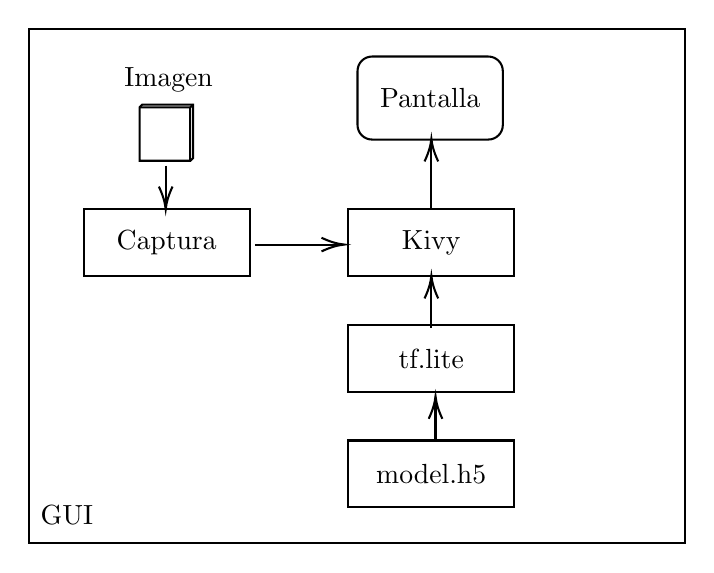
\begin{tikzpicture}[x=0.75pt,y=0.75pt,yscale=-1,xscale=1]
    %uncomment if require: \path (0,300); %set diagram left start at 0, and has height of 300
    
    %Flowchart: Process [id:dp38080226322023414] 
    \draw   (363.5,229) -- (443.5,229) -- (443.5,261.2) -- (363.5,261.2) -- cycle ;
    %Shape: Cube [id:dp8468046915311254] 
    \draw   (263,68.49) -- (264.29,67.2) -- (288.73,67.2) -- (288.73,92.91) -- (287.44,94.2) -- (263,94.2) -- cycle ; \draw   (288.73,67.2) -- (287.44,68.49) -- (263,68.49) ; \draw   (287.44,68.49) -- (287.44,94.2) ;
    %Flowchart: Process [id:dp3784953439432983] 
    \draw   (363.5,173.5) -- (443.5,173.5) -- (443.5,205.7) -- (363.5,205.7) -- cycle ;
    %Flowchart: Process [id:dp6706534673883591] 
    \draw   (236,117.5) -- (316,117.5) -- (316,149.7) -- (236,149.7) -- cycle ;
    %Flowchart: Alternative Process [id:dp06859905125399013] 
    \draw   (368,51) .. controls (368,47.13) and (371.13,44) .. (375,44) -- (431,44) .. controls (434.87,44) and (438,47.13) .. (438,51) -- (438,77) .. controls (438,80.87) and (434.87,84) .. (431,84) -- (375,84) .. controls (371.13,84) and (368,80.87) .. (368,77) -- cycle ;
    %Shape: Rectangle [id:dp8508559969443851] 
    \draw   (209.58,30.6) -- (525.58,30.6) -- (525.58,278.6) -- (209.58,278.6) -- cycle ;
    %Straight Lines [id:da7738568846869857] 
    \draw    (275.58,96.6) -- (275.58,115.6) ;
    \draw [shift={(275.58,117.6)}, rotate = 270] [color={rgb, 255:red, 0; green, 0; blue, 0 }  ][line width=0.75]    (10.93,-3.29) .. controls (6.95,-1.4) and (3.31,-0.3) .. (0,0) .. controls (3.31,0.3) and (6.95,1.4) .. (10.93,3.29)   ;
    
    %Straight Lines [id:da6265254082403638] 
    \draw    (403.58,174.6) -- (403.58,151.6) ;
    \draw [shift={(403.58,149.6)}, rotate = 450] [color={rgb, 255:red, 0; green, 0; blue, 0 }  ][line width=0.75]    (10.93,-3.29) .. controls (6.95,-1.4) and (3.31,-0.3) .. (0,0) .. controls (3.31,0.3) and (6.95,1.4) .. (10.93,3.29)   ;
    
    %Straight Lines [id:da5790227887597429] 
    \draw    (405.58,228.6) -- (405.58,209.6) ;
    \draw [shift={(405.58,207.6)}, rotate = 450] [color={rgb, 255:red, 0; green, 0; blue, 0 }  ][line width=0.75]    (10.93,-3.29) .. controls (6.95,-1.4) and (3.31,-0.3) .. (0,0) .. controls (3.31,0.3) and (6.95,1.4) .. (10.93,3.29)   ;
    
    %Straight Lines [id:da3353787323675512] 
    \draw    (318.58,134.6) -- (359.58,134.6) ;
    \draw [shift={(361.58,134.6)}, rotate = 180] [color={rgb, 255:red, 0; green, 0; blue, 0 }  ][line width=0.75]    (10.93,-3.29) .. controls (6.95,-1.4) and (3.31,-0.3) .. (0,0) .. controls (3.31,0.3) and (6.95,1.4) .. (10.93,3.29)   ;
    
    %Flowchart: Process [id:dp23423991466702976] 
    \draw   (363.5,117.5) -- (443.5,117.5) -- (443.5,149.7) -- (363.5,149.7) -- cycle ;
    %Straight Lines [id:da7698169631875084] 
    \draw    (403.58,117.6) -- (403.58,85.6) ;
    \draw [shift={(403.58,83.6)}, rotate = 450] [color={rgb, 255:red, 0; green, 0; blue, 0 }  ][line width=0.75]    (10.93,-3.29) .. controls (6.95,-1.4) and (3.31,-0.3) .. (0,0) .. controls (3.31,0.3) and (6.95,1.4) .. (10.93,3.29)   ;
    
    
    % Text Node
    \draw (277,55) node [scale=1] [align=left] {Imagen};
    % Text Node
    \draw (276,133.6) node  [align=left] {Captura};
    % Text Node
    \draw (403.5,245.1) node  [align=left] {model.h5};
    % Text Node
    \draw (403.5,189.6) node  [align=left] {tf.lite};
    % Text Node
    \draw (403,64) node  [align=left] {Pantalla};
    % Text Node
    \draw (228,265) node  [align=left] {GUI};
    % Text Node
    \draw (403.5,133.6) node  [align=left] {Kivy};
    
    
    \end{tikzpicture}
\caption{Diagrama general del sistema}\label{fig:diagrama_sistema}
\end{figure}

\subsubsection{Configuración de LINUX}

El proceso para instalar LINUX en Jetson nano es sencillo, hay que grabar el
sistema operativo en una memoria microSD para posteriormente insertarla en la
tarjeta. Los pasos son los siguientes (\autoref{fig:jetson_linux}):

\begin{enumerate}
    \item Descargar la imagen del sistema operativo personalizado de Nvidia.
    \item Formatear la tarjeta microSD.
    \item Escribir la imagen en la tarjeta microSD.
\end{enumerate}

\begin{figure}[H]
    \centering
    \includegraphics[width=\textwidth]{capitulo_sdac/jetson_linux.png}
    \caption{Linux personalizado de Nvidia en Jetson}\label{fig:jetson_linux}
\end{figure}

Luego de actualizar el sistema operativo. Se procede a instalar las dependencias
de Python para poder desarrollar el sistema. Debido a que la complejidad de
compilar \emph{OpenCV} es considerable, su instalación sale del espectro de esta
tesis, tardando su compilación hasta más de 5 horas y necesitando forzosamente
la modificación de parámetros internos de administración de memoria de la
tarjeta.

\subsubsection{Interface gráfica}

Para la interface gráfica necesitamos un framework capaz de hacer fácil el
desarrollo y que pueda ser desplegado en cualquier sistema operativo, también
tiene que tener funcionalidad táctil integrada.

Kivy es un módulo de Python para desarrollo rápido de aplicaciones que usan
interfaces innovadoras, como aquellas que requieren dispositivos táctiles. Kivy
puede ser usado en todos los sistemas operativos incluyendo el de Jetson Nano y
maneja muchos protocolos de ingreso de impulsos táctiles. Es 100\% libre bajo
una licencia del MIT y cuenta con desarrollo profesional. Analizando estos
argumento se concluye que Kivy es la única opción de framework para crear la
interface gráfica.

Kivy funciona dividiendo el desarrollo de la interface en dos capas. La primera
es aquella que provee la funcionalidad de backend, es decir, todo lo que va a
soportar la interface propiamente dicha. Esto se programa en lenguaje Python. La
segunda capa es la capa que describe como se va a renderizar la interface
gráfica en el dispositivo, para ello se hace uso de un lenguaje de marcado
específico con extensión \emph{.kv}.

La arquitectura de Kivy, \autoref{fig:kivy} va desde el bajo nivel, compuesto de
módulos y \emph{drivers} tanto externos como del sistema operativo; los módulos
usados para la creación de la interface son GStreamer para la cámara o WM\_Touch
para la entrada de datos táctiles. Al centro encontramos los elementos para
armar la interface, por ejemplo, ventanas o imágenes; también maneja la parte
gráfica y direcciona las entradas al \emph{driver} correspondiente. El alto
nivel contiene el lenguaje \emph{.kv} y las funciones para crear la app en su noción
general.

\begin{figure}[H]
    \centering
    \includegraphics[width=0.6\textwidth]{capitulo_sdac/kivy}
    \caption{La arquitectura de Kivy}\label{fig:kivy}
\end{figure}

Toda la lógica para soportar la captura de imagen y alimentar el modelo se hace
en Python y es directamente integrada con Kivy. Mientras que el lenguaje \emph{.kv} y
el módulo abstraen toda la parte de la generación de la interface y la forma en
que se conecta al software de la tarjeta que maneja la pantalla táctil. Esto
hace el desarrollo sumamente sencillo\footnote{Elegir las tecnologías correctas simplifica
mucho cualquier desarrollo tecnológico}.

En la \autoref{fig:gui} tenemos un ejemplo de pantalla principal para el
sistema. Esta interface es sencilla y fácil de usar. Una vez presionado el botón
correspondiente nos dirigirá a la siguiente ventana para utilizar la inferencia.

\begin{figure}[]
    \centering
    \includegraphics[width=0.9\textwidth]{capitulo_sdac/gui}
    \caption{Linux personalizado de Nvidia en Jetson}\label{fig:gui}
\end{figure}

Para la inferencia (\autoref{fig:gui2}) podemos cargar una imagen o alimentarla
desde el microscopio. La célula se muestra en pantalla y posterior activación
del botó indicado, se procesa y genera una gráfica de barras; donde se indica la
probabilidad de pertenecer a alguna de las siete clases.

\begin{figure}[]
    \centering
    \includegraphics[width=0.9\textwidth]{capitulo_sdac/gui2}
    \caption{Linux personalizado de Nvidia en Jetson}\label{fig:gui2}
\end{figure}

% \subsubsection{Captura de imagen}

\subsection{Sistema}

Se culmina el diseño conceptual mediante la integración del módulo de
\hyperlink{abbr}{ConvNet}, la interface gráfica y la Jetson Nano. Para el primer
prototipo se logró instalar todas las dependencias de Linux, OpenCV para la
captura de imagen y configurar tanto el intérprete de Python como la captura de
pantalla táctil mediante el \emph{Driver} de la placa Jetson Nano y la pantalla.

Optimizaciones posteriores del \emph{Kernel} del sistema operativo así como la
instalación de módulos adicionales para cómputo tensorial (TensorRT) son
necesarios para proseguir con las pruebas del motor de inferencia.

En la \autoref{fig:prototipo_final} podemos observar la pantalla conectada a la
Jetson mostrando la interface gráfica creada para el sistema. No se muestra
puntero en la pantalla ya que todo el control es mediante impulsos táctiles.

\begin{figure}[]
    \centering
    \includegraphics[width=\textwidth]{capitulo_sdac/prototipo_final}
    \caption{Muestra del prototipo con la interface del sistema}\label{fig:prototipo_final}
\end{figure}
